% Book 4, Year 2, chapter 25 -- Text algorithms and compression.
% Provenance (never printed): sources/book4/BRIEFS.md, chapter 25.
\chapter{Text Algorithms and Compression}\label{ch:b2:text-algorithms}

The town keeps an archive: a line for every loan, every return and every weather reading of the year, 87,299
characters. Finding a phrase in it is the oldest text problem, and three algorithms solve it with very different
amounts of work:

\omcode{code/bachelor-2/25-text-algorithms/listings/search.py}{7}{14}{Two phrases looked for in the archive by the naive
search, by Boyer--Moore and by Knuth--Morris--Pratt, counting letter comparisons}\label{lst:b2:text-algorithms:search}

\omoutput{code/bachelor-2/25-text-algorithms/outputs/search.txt}{The same \omterm{def:b2:text-algorithms:matching}{occurrences}, three costs: Boyer--Moore looks at
about one letter in ten.}\label{out:b2:text-algorithms:search}

The naive search and KMP look at about one comparison per letter of the text, Boyer--Moore at a tenth of that. Yet the
naive search can be forced into $m$ comparisons per letter for a pattern of $m$ letters, and KMP never makes more than
two. This chapter proves these costs, adds a search by hashing and a tree of words for completing names, and ends with
the other thing one does with an archive: store it in less space.

\begin{recall}
The grade 12 volume: a pattern and its \omterm{def:b2:text-algorithms:matching}{occurrences} in a text, the naive search, Horspool's shift table. \Cref{ch:b2:finite-automata}:
deterministic finite automata. The Year 1 volume: Huffman codes, the optimal prefix code for given letter frequencies;
hash functions and hash tables; the potential method of amortised analysis, in which a quantity that never goes below
zero pays for expensive steps.
\end{recall}

\section{String matching}\label{sec:b2:text-algorithms:matching}

\begin{definition}[String matching, occurrence, shift]\label{def:b2:text-algorithms:matching}
Let $T = T[0..n-1]$ be a \emph{text} and $P = P[0..m-1]$ a \emph{pattern}, words over an \omterm{def:b2:finite-automata:word}{alphabet} $\Sigma$, with $1 \leq
m$. A \emph{shift} is an integer $s$ with $0 \leq s \leq n - m$; it is an \emph{occurrence}\index{occurrence (string
matching)} of $P$ when $T[s + j] = P[j]$ for $0 \leq j < m$. \emph{String matching}\index{string matching} is the problem
of finding every occurrence.
\end{definition}

The cost measure in this chapter is the number of comparisons of two letters, which the listings count.

\omcode{code/bachelor-2/25-text-algorithms/listings/naive.py}{4}{16}{The naive search: every shift, letters compared
from the left until a difference}\label{lst:b2:text-algorithms:naive}

\begin{proposition}[Cost of the naive search]\label{prop:b2:text-algorithms:naive}
The naive search makes at most $m(n - m + 1)$ comparisons, and exactly that many on the text $a^n$ with the pattern
$a^{m-1}b$.
\end{proposition}

\begin{proof}
Each of the $n - m + 1$ shifts compares at most $m$ letters. On $a^n$ with $a^{m-1}b$, every shift matches $m - 1$
letters and fails on the last, so it makes exactly $m$ comparisons.
\end{proof}

On ordinary text the first comparison of a shift usually fails, and the cost is close to $n$, as in
\cref{out:b2:text-algorithms:search}. The worst case is not exotic, though: a log file of repeated lines, a DNA
sequence or a binary file are close to it.

\section{Boyer--Moore and the bad-character rule}\label{sec:b2:text-algorithms:boyer-moore}

The grade 12 volume compared the pattern from its right end and jumped with a table of letters. The same idea, made
exact:

\begin{definition}[Bad-character rule]\label{def:b2:text-algorithms:bad-char}
Compare $P$ with the text at shift $s$ from the right, and let $j$ be the position of the first difference, with $c =
T[s + j]$ the \emph{bad character}. Let $\lambda(c)$ be the last position of $c$ in $P$, or $-1$ if $c$ does not occur
in $P$. The \emph{bad-character rule}\index{bad-character rule} moves to the shift $s + \max(1, j - \lambda(c))$.
\end{definition}

\begin{omfigure}
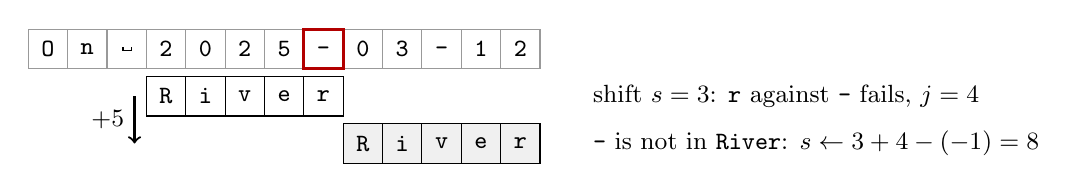
\begin{tikzpicture}[x=5mm, y=5mm, every node/.style={font=\ttfamily\small}]
\foreach \c [count=\i from 0] in {O,n,\textvisiblespace,2,0,2,5,-,0,3,-,1,2} {
  \node[draw=black!40, minimum size=5mm, inner sep=0pt] at (\i, 2) {\c};
}
\foreach \c [count=\i from 3] in {R,i,v,e,r} {
  \node[draw, minimum size=5mm, inner sep=0pt] at (\i, 0.8) {\c};
}
\node[draw=red!70!black, very thick, minimum size=5mm] at (7, 2) {};
\foreach \c [count=\i from 8] in {R,i,v,e,r} {
  \node[draw, fill=black!6, minimum size=5mm, inner sep=0pt] at (\i, -0.4) {\c};
}
\draw[->, thick] (2.2, 0.8) -- (2.2, -0.4) node[midway, left, font=\small] {$+5$};
\node[anchor=west, font=\small] at (13.6, 0.8) {shift $s = 3$: \texttt{r} against \texttt{-} fails, $j = 4$};
\node[anchor=west, font=\small] at (13.6, -0.4) {\texttt{-} is not in \texttt{River}: $s \gets 3 + 4 - (-1) = 8$};
\end{tikzpicture}
\par\smallskip{\small The \omterm{def:b2:text-algorithms:bad-char}{bad-character rule}. The pattern \texttt{River} is compared from its right end; the text's
\texttt{-} differs from \texttt{r} and occurs nowhere in the pattern, so no shift that puts a letter of the pattern under
it can match, and the pattern jumps past it.}
\end{omfigure}

\begin{proposition}[No occurrence is skipped]\label{prop:b2:text-algorithms:bad-char}
The \omterm{def:b2:text-algorithms:bad-char}{bad-character rule} never jumps over an \omterm{def:b2:text-algorithms:matching}{occurrence}: no shift $s'$ with $s < s' < s + \max(1, j - \lambda(c))$ is an
\omterm{def:b2:text-algorithms:matching}{occurrence}.
\end{proposition}

\begin{proof}
A shift $s' = s + d$ with $0 < d < j - \lambda(c)$ puts the pattern's position $j - d$ under the text position $s + j$,
which holds $c$. Since $j - d > \lambda(c)$, and $\lambda(c)$ is the last position of $c$ in $P$, $P[j - d] \neq c$: the
shift $s'$ is not an \omterm{def:b2:text-algorithms:matching}{occurrence}. If $j - \lambda(c) \leq 1$, the rule moves by $1$ and skips nothing.
\end{proof}

\omcode{code/bachelor-2/25-text-algorithms/listings/boyer_moore.py}{4}{26}{Boyer--Moore with the \omterm{def:b2:text-algorithms:bad-char}{bad-character rule}}\label{lst:b2:text-algorithms:boyer-moore}

When the bad character does not occur in the pattern, the jump is $j + 1$, up to $m$; on ordinary text with a long
pattern, most shifts are skipped unread, which explains the tenfold saving of \cref{out:b2:text-algorithms:search}. The
worst case is still $m(n - m + 1)$, on $a^n$ with $ba^{m-1}$. Boyer and Moore's algorithm adds a second rule, the
\emph{good \omterm{def:b2:finite-automata:factor}{suffix}}, which uses the part already matched; with it the worst case becomes linear. KMP reaches that bound
with the matched part alone, and from the left.

\section{Knuth--Morris--Pratt}\label{sec:b2:text-algorithms:kmp}

When the naive search fails after matching $q$ letters, it starts again one letter further and reads again text that it
has already seen. Those $q$ letters are known: they are $P[0..q-1]$. Which shifts can still succeed depends only on the
pattern.

\begin{definition}[Border, failure function]\label{def:b2:text-algorithms:border}
A \emph{border}\index{border (word)} of a word $u$ is a word that is both a proper prefix and a proper \omterm{def:b2:finite-automata:factor}{suffix} of $u$
(the \omterm{def:b2:finite-automata:word}{empty word} is always one). The \emph{failure function}\index{failure function} of $P$ is $\pi(q)$, the length of the
longest border of $P[0..q-1]$, for $1 \leq q \leq m$.
\end{definition}

\begin{omfigure}
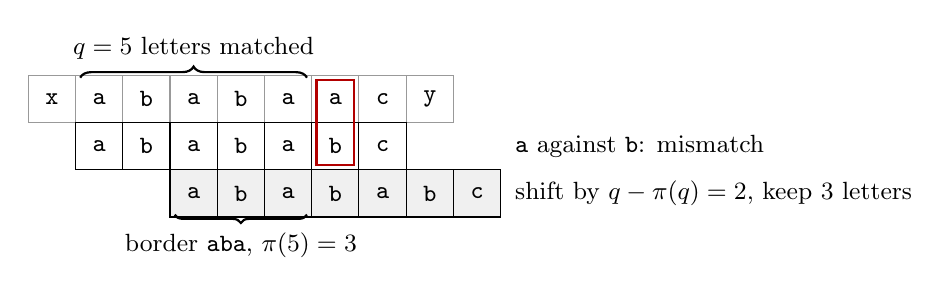
\begin{tikzpicture}[x=6mm, y=6mm, every node/.style={font=\ttfamily\small}]
\foreach \c [count=\i from 0] in {x,a,b,a,b,a,a,c,y} {
  \node[draw=black!40, minimum size=6mm, inner sep=0pt] at (\i, 2) {\c};
}
\foreach \c [count=\i from 1] in {a,b,a,b,a,b,c} {
  \node[draw, minimum size=6mm, inner sep=0pt] at (\i, 1) {\c};
}
\foreach \c [count=\i from 3] in {a,b,a,b,a,b,c} {
  \node[draw, fill=black!6, minimum size=6mm, inner sep=0pt] at (\i, 0) {\c};
}
\draw[decorate, decoration={brace, amplitude=4pt}, thick] (0.6, 2.45) -- (5.4, 2.45)
  node[midway, above=3pt, font=\small] {$q = 5$ letters matched};
\draw[thick, red!70!black] (5.6, 0.6) rectangle (6.4, 2.4);
\draw[decorate, decoration={brace, amplitude=3pt, mirror}, thick] (2.6, -0.45) -- (5.4, -0.45)
  node[midway, below=3pt, font=\small] {border \texttt{aba}, $\pi(5) = 3$};
\node[anchor=west, font=\small] at (9.6, 1) {\texttt{a} against \texttt{b}: mismatch};
\node[anchor=west, font=\small] at (9.6, 0) {shift by $q - \pi(q) = 2$, keep $3$ letters};
\end{tikzpicture}
\par\smallskip{\small A mismatch after $q = 5$ letters of \texttt{abababc}. The matched part \texttt{ababa} has the
longest \omterm{def:b2:text-algorithms:border}{border} \texttt{aba}; the pattern moves so that its prefix \texttt{aba} sits under the text's \texttt{aba}, and
the comparison resumes at the same text letter, with $q = 3$.}
\end{omfigure}

If $P[0..q-1]$ matches the text up to position $i - 1$ and $P[q] \neq T[i]$, a shift by $d$ with $0 < d < q$ can only
succeed if $P[0..q-d-1] = P[d..q-1]$, that is if $P[0..q-d-1]$ is a \omterm{def:b2:text-algorithms:border}{border} of $P[0..q-1]$. The smallest useful shift
keeps the longest \omterm{def:b2:text-algorithms:border}{border}: the new $q$ is $\pi(q)$, and the text letter $T[i]$ is compared again.

\begin{method}[Knuth--Morris--Pratt]\label{met:b2:text-algorithms:kmp}
Compute $\pi$. Then read the text once, keeping $q$, the number of pattern letters matched. For each text letter $c$:
while $q > 0$ and $P[q] \neq c$, set $q \gets \pi(q)$; if $P[q] = c$, increase $q$. When $q = m$, report the \omterm{def:b2:text-algorithms:matching}{occurrence}
ending here and set $q \gets \pi(m)$. Stop when the pattern, placed at shift $i - q$, no longer fits in the
text.\index{Knuth--Morris--Pratt algorithm}
\end{method}

\omcode{code/bachelor-2/25-text-algorithms/listings/kmp.py}{5}{37}{The \omterm{def:b2:text-algorithms:border}{failure function} and the KMP search; the text
index $i$ only moves forwards}\label{lst:b2:text-algorithms:kmp}

\omoutput{code/bachelor-2/25-text-algorithms/outputs/kmp.txt}{\omterm{def:b2:text-algorithms:border}{Failure functions}, written $q{:}\pi(q)$. A pattern with
no repeated prefix, such as a date, has $\pi = 0$ everywhere.}\label{out:b2:text-algorithms:kmp}

The \omterm{def:b2:text-algorithms:border}{failure function} is computed by the same search, run on the pattern against itself: \code{k} is the longest \omterm{def:b2:text-algorithms:border}{border}
of the prefix read so far, extended by one letter when the next letters agree, and shortened along the chain $k, \pi(k),
\pi(\pi(k)), \dots$ of ever shorter \omterm{def:b2:text-algorithms:border}{borders} otherwise. The chain lists all \omterm{def:b2:text-algorithms:border}{borders}, because a \omterm{def:b2:text-algorithms:border}{border} of a \omterm{def:b2:text-algorithms:border}{border} of $u$
is a \omterm{def:b2:text-algorithms:border}{border} of $u$, and the longest \omterm{def:b2:text-algorithms:border}{border} shorter than $\pi(q)$ is $\pi(\pi(q))$.

\begin{proposition}[The failure function in linear time]\label{prop:b2:text-algorithms:failure}
\code{failure} computes $\pi$ in $\BigO(m)$ steps.
\end{proposition}

\begin{proof}
Correctness: if $P[0..q-1]$ has a \omterm{def:b2:text-algorithms:border}{border} of length $k + 1 \geq 1$, removing its last letter gives a \omterm{def:b2:text-algorithms:border}{border} of length $k$
of $P[0..q-2]$ followed by $P[k] = P[q - 1]$; trying the \omterm{def:b2:text-algorithms:border}{borders} of $P[0..q-2]$ from the longest, the first one so
extended is the longest \omterm{def:b2:text-algorithms:border}{border} of $P[0..q-1]$. Cost: $k$ increases by at most $1$ for each $q$, so at most $m - 1$
times in all; each iteration of the inner loop decreases $k$ and $k \geq 0$, so the inner loop runs at most $m - 1$
times in all.
\end{proof}

\begin{theorem}[KMP is linear]\label{thm:b2:text-algorithms:kmp-linear}
The search of \cref{lst:b2:text-algorithms:kmp} makes at most $2n - m$ comparisons on a text of length $n \geq m$.
\end{theorem}

\begin{proof}
When the letter $T[i]$ is compared with $P[q]$, the pattern is at the shift $s = i - q$. Consider the sum $i + s$. A
comparison that succeeds increases $q$ and then $i$ (the loop moves to the next letter): $i$ grows by $1$ and $s$ is
unchanged. A failure with $q = 0$ moves to the next letter with $q = 0$: $i$ and $s$ both grow by $1$. A failure with
$q > 0$ replaces $q$ by $\pi(q) < q$ at the same $i$: $s$ grows. So between two comparisons $i + s$ increases by at least
$1$. Every comparison happens with $i \leq n - 1$ and $s \leq n - m$, the program stopping before any other, so $i + s$
takes at most the values $0, 1, \dots, 2n - m - 1$ at comparisons: at most $2n - m$ of them.
\end{proof}

The argument is a potential argument with the potential $i + s$, and it bounds the total work without bounding the work
on one letter: one text letter may be compared many times, as the chain of \omterm{def:b2:text-algorithms:border}{borders} is followed, but each of those
comparisons moves the pattern forward for good.

\begin{definition}[String-matching automaton]\label{def:b2:text-algorithms:automaton}
The \emph{string-matching automaton}\index{string-matching automaton} of $P$ over $\Sigma$ is the DFA with states $0,
\dots, m$, start state $0$, \omterm{def:b2:finite-automata:dfa}{accepting state} $m$, and transition $\delta(q, c)$ the length of the longest prefix of $P$
that is a \omterm{def:b2:finite-automata:factor}{suffix} of $P[0..q-1]c$.
\end{definition}

The automaton reads the text once, one transition per letter, and is in state $m$ exactly at the end of each \omterm{def:b2:text-algorithms:matching}{occurrence}.
It is KMP with every chain of \omterm{def:b2:text-algorithms:border}{borders} followed in advance: $\delta(q, c) = q + 1$ when $P[q] = c$, and otherwise
$\delta(q, c) = \delta(\pi(q), c)$, or $0$ from state $0$.

\omcode{code/bachelor-2/25-text-algorithms/listings/kmp_automaton.py}{6}{27}{The automaton from the \omterm{def:b2:text-algorithms:border}{failure function}, and
a run that costs one lookup per letter}\label{lst:b2:text-algorithms:automaton}

\omoutput{code/bachelor-2/25-text-algorithms/outputs/kmp_automaton.txt}{The transition table of \texttt{ababc} over
$\{a, b, c\}$, and the two \omterm{def:b2:text-algorithms:matching}{occurrences} in a text.}\label{out:b2:text-algorithms:automaton}

\begin{omfigure}
\begin{tikzpicture}[>=stealth, node distance=16mm, every state/.style={minimum size=7mm, inner sep=1pt}, thick]
\node[state, initial, initial text=] (q0) {$0$};
\node[state, right=of q0] (q1) {$1$};
\node[state, right=of q1] (q2) {$2$};
\node[state, right=of q2] (q3) {$3$};
\node[state, right=of q3] (q4) {$4$};
\node[state, accepting, right=of q4] (q5) {$5$};
\draw[->] (q0) -- node[above] {a} (q1);
\draw[->] (q1) -- node[above] {b} (q2);
\draw[->] (q2) -- node[above] {a} (q3);
\draw[->] (q3) -- node[above] {b} (q4);
\draw[->] (q4) -- node[above] {c} (q5);
\draw[->] (q1) edge[loop above] node {a} (q1);
\draw[->] (q3) to[bend right=40] node[above] {a} (q1);
\draw[->] (q4) to[bend left=40] node[below] {a} (q3);
\draw[->] (q5) to[bend left=35] node[below] {a} (q1);
\end{tikzpicture}
\par\smallskip{\small The \omterm{def:b2:text-algorithms:automaton}{string-matching automaton} of \texttt{ababc}, drawn from \cref{out:b2:text-algorithms:automaton}.
The edges not drawn lead to state $0$. From state $4$ (\texttt{abab} read), an \texttt{a} leads to $3$: \texttt{ababa}
ends with \texttt{aba}.}
\end{omfigure}

The table has $(m + 1)|\Sigma|$ entries. For bytes that is $256$ columns, which is why programs usually keep the \omterm{def:b2:text-algorithms:border}{failure
function}, of size $m$, and follow it at run time.

\begin{history}
% ledger: b2:kmp-1977
% ledger: b2:boyer-moore-1977
Donald Knuth, James Morris and Vaughan Pratt published their algorithm in 1977; the same year Robert Boyer and J
Strother Moore published the search from the right with its two rules.
\end{history}

\section{Rabin--Karp}\label{sec:b2:text-algorithms:rabin-karp}

Comparing letters is not the only way to compare words. A word of $m$ letters is a number in base $256$, and two equal
words give equal numbers; reduced modulo a prime $q$, the numbers are small, and the number of the next window is
computed from the current one in constant time.

\begin{definition}[Rolling hash, spurious hit]\label{def:b2:text-algorithms:rolling}
The \emph{rolling hash}\index{rolling hash} of a window $T[s..s+m-1]$ is $h_s = \sum_{j=0}^{m-1} T[s + j]\, 256^{m-1-j}
\bmod q$. It satisfies $h_{s+1} = ((h_s - T[s] \cdot 256^{m-1}) \cdot 256 + T[s + m]) \bmod q$. A shift whose hash equals
the pattern's, $h_s = h(P)$, but which is not an \omterm{def:b2:text-algorithms:matching}{occurrence}, is a \emph{spurious hit}\index{spurious hit}.
\end{definition}

\begin{method}[Rabin--Karp]\label{met:b2:text-algorithms:rabin-karp}
Compute $h(P)$ and $h_0$, then $h_1, h_2, \dots$ by the rolling formula. At each shift with $h_s = h(P)$, compare the
window with $P$ letter by letter: report it if they agree, count a \omterm{def:b2:text-algorithms:rolling}{spurious hit}
otherwise.\index{Rabin--Karp algorithm}
\end{method}

\omcode{code/bachelor-2/25-text-algorithms/listings/rabin_karp.py}{7}{26}{Rabin--Karp: one multiplication and one
addition per shift, and a check on equal hashes}\label{lst:b2:text-algorithms:rabin-karp}

\begin{proposition}[Expected spurious hits]\label{prop:b2:text-algorithms:spurious}
If every window different from $P$ has $h_s = h(P)$ with probability at most $1/q$, the expected number of \omterm{def:b2:text-algorithms:rolling}{spurious
hits} is at most $(n - m + 1)/q$, and the expected cost of the checks on them at most $m(n - m + 1)/q$.
\end{proposition}

\begin{proof}
The number of \omterm{def:b2:text-algorithms:rolling}{spurious hits} is a sum over the $n - m + 1$ shifts of indicator variables, each of expectation at most
$1/q$; the expectation of a sum is the sum of the expectations. Each \omterm{def:b2:text-algorithms:rolling}{spurious hit} costs at most $m$ comparisons.
\end{proof}

The hypothesis is a model, not a theorem about a fixed $q$: a text could be built to collide with the pattern for one
modulus. Karp and Rabin choose the prime at random, and then the bound is proved
(\cref{exo:b2:text-algorithms:10}). In practice the model is close:

\omoutput{code/bachelor-2/25-text-algorithms/outputs/rk_demo.txt}{\omterm{def:b2:text-algorithms:rolling}{Spurious hits} on the archive. With $q = 97$, hundreds,
near the model's estimate $(n - m + 1)/q$; with $q = 1{,}000{,}003$, none.}\label{out:b2:text-algorithms:rk}

Rabin--Karp is slower than KMP for one pattern, but it extends at no cost to many patterns of the same length: put
their hashes in a hash table, and check the windows whose hash is in it (\cref{exo:b2:text-algorithms:9}). It also
compares other objects than words, such as the blocks of two files.

% ledger: b2:karp-rabin-1987
Richard Karp and Michael Rabin published the method in 1987, with a random prime as the modulus.

\section{Tries}\label{sec:b2:text-algorithms:tries}

Completing a name as it is typed asks for every word of a set that starts with a given prefix. Sorting the words and
searching by halves answers it; a tree indexed by letters answers it in time that depends on the prefix, not on the
size of the set.

\begin{definition}[Trie]\label{def:b2:text-algorithms:trie}
A \emph{trie}\index{trie} of a finite set of words is a rooted tree whose edges are labelled by letters, the edges out
of a node having distinct labels, with a mark on some nodes: the word spelled from the root to a node is in the set
exactly when the node is marked, and every leaf is marked.
\end{definition}

\omcode{code/bachelor-2/25-text-algorithms/listings/trie.py}{4}{38}{A \omterm{def:b2:text-algorithms:trie}{trie}: each node maps letters to subtries; the
words under a prefix in alphabetical order}\label{lst:b2:text-algorithms:trie}

\begin{proposition}[Trie operations]\label{prop:b2:text-algorithms:trie}
A \omterm{def:b2:text-algorithms:trie}{trie} of words of total length $L$ has at most $L + 1$ nodes. Inserting or finding a word of length $k$ takes $k$
lookups in the children's tables; listing the $r$ words that start with a prefix $u$ takes $|u|$ lookups and a walk of
the subtrie below $u$, whose size is at most the total length of those $r$ words plus one.
\end{proposition}

\begin{proof}
Each node except the root is created by one letter of one inserted word, so there are at most $L$ of them. Insertion and
search follow one edge per letter. The words under $u$ are those spelled by the marked nodes of the subtrie at $u$, and
each node of that subtrie lies on the path of at least one of them.
\end{proof}

\omoutput{code/bachelor-2/25-text-algorithms/outputs/trie_demo.txt}{The 24 street names in 164 nodes instead of 258
letters, completions, and the compressed \omterm{def:b2:text-algorithms:trie}{trie} of eight names.}\label{out:b2:text-algorithms:trie}

\begin{omfigure}
\forestset{el/.style={edge label={node[pos=0.72, fill=white, font=\ttfamily\scriptsize, inner sep=1pt]{#1}}}}
\begin{forest}
for tree={font=\small, l sep=30pt, s sep=36pt, circle, draw, minimum size=3mm, inner sep=0pt}
[
  [, el={Castle\textvisiblespace}
    [, el={Ro} [, fill=black, el={ad}] [, fill=black, el={w}]]
    [, fill=black, el={Way}]]
  [, el={M}
    [, el={arket\textvisiblespace Ro} [, fill=black, el={ad}] [, fill=black, el={w}]]
    [, el={ill\textvisiblespace} [, fill=black, el={Avenue}] [, fill=black, el={Row}]
      [, fill=black, el={Street}]]]]
\end{forest}
\par\smallskip{\small The compressed \omterm{def:b2:text-algorithms:trie}{trie} of eight street names, printed by \cref{out:b2:text-algorithms:trie}: each chain
of single children is one edge labelled by a word. A filled node ends a name. The \omterm{def:b2:text-algorithms:trie}{trie} itself has 47 nodes, this one
14.}
\end{omfigure}

In a \emph{compressed \omterm{def:b2:text-algorithms:trie}{trie}} (also called a radix tree) every node has two children or more, or ends a word, so the
number of nodes is at most twice the number of words. A \omterm{def:b2:text-algorithms:trie}{trie} of patterns with, at each node, a link to the longest
\omterm{def:b2:finite-automata:factor}{suffix} of its word that is also a node finds every \omterm{def:b2:text-algorithms:matching}{occurrence} of many patterns in one pass over a text, the way KMP
does for one (\cref{exo:b2:text-algorithms:11}).

\section{Compression: Lempel--Ziv--Welch}\label{sec:b2:text-algorithms:lzw}

A Huffman code gives each byte a code word of a length that suits its frequency. The archive repeats whole words,
``borrowed'', ``returned'', ``degrees and'', which a code for single bytes cannot exploit. A \omterm{def:b2:text-algorithms:lzw}{dictionary coder} codes
the repeated words themselves.

\begin{definition}[Dictionary coder, Lempel--Ziv--Welch coding]\label{def:b2:text-algorithms:lzw}
A \emph{dictionary coder}\index{dictionary coder} replaces pieces of the input by their numbers in a dictionary of
words. \emph{Lempel--Ziv--Welch coding}\index{Lempel--Ziv--Welch coding} (LZW) starts with the dictionary of the 256 single
bytes, numbered $0$ to $255$. It repeatedly reads the longest word $w$ of the dictionary that the input starts with,
emits its number, and adds to the dictionary $w$ followed by the next byte of the input, under the next free number.
\end{definition}

The dictionary is not sent. The decoder builds the same one as it reads the codes, one entry behind: when it reads a
code, it knows the word just decoded and the first byte of the new one, which is what the encoder added.

\omcode{code/bachelor-2/25-text-algorithms/listings/lzw.py}{4}{39}{LZW: the encoder, and the decoder that rebuilds its
dictionary, with the code that is not yet in it}\label{lst:b2:text-algorithms:lzw}

\omoutput{code/bachelor-2/25-text-algorithms/outputs/lzw_demo.txt}{LZW on two short texts. In \texttt{abababa} the
last code, 258, is used by the encoder right after creating it.}\label{out:b2:text-algorithms:lzw}

\begin{theorem}[The decoder rebuilds the dictionary]\label{thm:b2:text-algorithms:lzw}
On the codes emitted by the encoder, the decoder outputs the input. Before it reads the $(k+1)$-st code, $k \geq 1$, its
table holds the $256 + k - 1$ entries that the encoder's held when it emitted the $k$-th code.
\end{theorem}

\begin{proof}
Let $w_1, w_2, \dots$ be the words whose codes the encoder emits, in order; the input is their concatenation. The encoder
adds the entry $256 + k - 1$ as $w_k$ followed by the next input byte, which is the first byte of $w_{k+1}$, at the
moment it emits the code of $w_k$. By induction on $k$, assume the decoder has output $w_1, \dots, w_k$ and that its
table holds the entries up to $256 + k - 2$, the encoder's when it emitted $w_k$; this holds for $k = 1$. The encoder
emitted the code of $w_{k+1}$ with entries up to $256 + k - 1$, so the code is at most $256 + k - 1$. If it is smaller,
the decoder's table holds it and gives $w_{k+1}$. If it equals $256 + k - 1$, the entry the decoder does not have yet,
then $w_{k+1}$ is $w_k$ followed by the first byte of $w_{k+1}$; that byte is then the first byte of $w_k$, so $w_{k+1}
= w_k\, w_k[0]$, which is what the decoder computes. In both cases it then adds $w_k$ followed by the first byte of
$w_{k+1}$, the entry $256 + k - 1$ of the encoder.
\end{proof}

The special case happens whenever the input contains $x\,v\,x\,v\,x$ with $x$ a byte and $xv$ in the dictionary, as in
$abababa$; a decoder without it works on most inputs and fails on these (\cref{exo:b2:text-algorithms:6}).

\omoutput{code/bachelor-2/25-text-algorithms/outputs/ratio.txt}{The archive compressed three ways. Huffman codes bytes;
LZW, with each code written on just enough bits for the dictionary's size, codes repeated words; zlib combines
both.}\label{out:b2:text-algorithms:ratio}

Huffman saves the bytes' unequal frequencies: 63 distinct bytes need about 5 bits each. LZW saves the repetitions, and
its gain grows with the text, as its dictionary learns the archive's phrases (\cref{pb:b2:text-algorithms:1}).

\begin{inpractice}
% ledger: b2:welch-1984
% ledger: b2:ziv-lempel-1978
% ledger: b2:deflate
Terry Welch described LZW in 1984, as a variant of the dictionary method that Jacob Ziv and Abraham Lempel published
in 1978. The \code{zlib} library writes DEFLATE, which combines LZ77, a coder that
replaces a repeated piece by a reference to its previous \omterm{def:b2:text-algorithms:matching}{occurrence} (a distance and a length), with Huffman codes for
those references and for the bytes; it compresses the archive almost twice as well as LZW.
\end{inpractice}

\section{The cost on a hostile text}\label{sec:b2:text-algorithms:hostile}

The comparisons of \cref{prop:b2:text-algorithms:naive,thm:b2:text-algorithms:kmp-linear} turn into time. The same two
searches in C, on the text $a^n$ with the pattern $a^{99}b$:

\omoutput{code/bachelor-2/25-text-algorithms/outputs/kmp_bench.txt}{Measured on the author's laptop: comparisons are
exactly $m(n - m + 1)$ and $2n - m$, for $m = 100$; times are the best of three
runs.}\label{out:b2:text-algorithms:bench}

\begin{omfigure}
\begin{tikzpicture}
\begin{axis}[omrecord, width=0.72\linewidth, height=5cm, xlabel={text length $n$ (millions of letters)},
    ylabel={time (ms)}, xmin=0, xmax=1.7, ymin=0, ymax=60, legend style={font=\scriptsize}, legend pos=north west]
  \addplot[omDef, thick, mark=*, mark size=1pt] table[x expr=\thisrow{n}/1e6, y=naive]
    {code/bachelor-2/25-text-algorithms/figures/kmp_bench.dat};
  \addlegendentry{naive, $m(n - m + 1)$ comparisons}
  \addplot[omThm, thick, mark=square*, mark size=1pt] table[x expr=\thisrow{n}/1e6, y=kmp]
    {code/bachelor-2/25-text-algorithms/figures/kmp_bench.dat};
  \addlegendentry{KMP, $2n - m$ comparisons}
\end{axis}
\end{tikzpicture}
\par\smallskip{\small Both costs are linear in $n$ for a fixed pattern, with slopes in the ratio of about $m/2$: the
naive search pays for every letter of the pattern at every shift, KMP for at most two comparisons per text letter.}
\end{omfigure}

The ratio of the times, about 33, is smaller than the ratio of the comparisons, 50: KMP's loop does more work around
each comparison. For a fixed pattern the naive search is still linear in $n$; what grows without bound is the factor $m$,
and patterns of a thousand letters make it a thousand.

\section{Exercises}\label{sec:b2:text-algorithms:exercises}

\begin{exercise}[$\star$]\label{exo:b2:text-algorithms:1}
Compute the \omterm{def:b2:text-algorithms:border}{failure function} of \texttt{aabaaab} by hand, then check with \code{exo_failure.py}.
\end{exercise}

\begin{exercise}[$\star$]\label{exo:b2:text-algorithms:2}
The function \code{kmp_short} of \code{exo_kmp_bug.py} is a shorter KMP: on a mismatch it sets $q \gets \pi(q)$ and moves
to the next letter. On which texts does it miss an \omterm{def:b2:text-algorithms:matching}{occurrence}? Correct it.
\end{exercise}

\begin{exercise}[$\star$]\label{exo:b2:text-algorithms:3}
After an \omterm{def:b2:text-algorithms:matching}{occurrence}, \cref{lst:b2:text-algorithms:boyer-moore} moves by one. Prove that moving by $m - \pi(m)$ skips no
\omterm{def:b2:text-algorithms:matching}{occurrence}, implement it, and compare the comparisons made on \texttt{abababababa} with \texttt{aba}, on $a^{30}$ with
$a^5$, and on the archive.
\end{exercise}

\begin{exercise}[$\star$]\label{exo:b2:text-algorithms:4}
Count the comparisons of the naive search on $a^n$ with $a^{m-1}b$, and on $a^n$ with $ba^{m-1}$. Do the same for
Boyer--Moore with the \omterm{def:b2:text-algorithms:bad-char}{bad-character rule}.
\end{exercise}

\begin{exercise}[$\star\star$]\label{exo:b2:text-algorithms:5}
Encode \texttt{she sells sea shells} with LZW by hand: list the codes and the entries added. Check with
\code{exo_lzw.py}.
\end{exercise}

\begin{exercise}[$\star\star$]\label{exo:b2:text-algorithms:6}
The decoder of \code{exo_lzw_bug.py} looks every code up in its table. On which of its three inputs does it fail, and
why? Characterise the inputs on which it fails.
\end{exercise}

\begin{exercise}[$\star\star$]\label{exo:b2:text-algorithms:7}
Write \code{first_k(trie, prefix, k)}, which returns the first $k$ words in alphabetical order that start with
\code{prefix} and stops as soon as it has them. Count the nodes it visits on the book titles.
\end{exercise}

\begin{exercise}[$\star\star$]\label{exo:b2:text-algorithms:8}
Show that the bound of \cref{thm:b2:text-algorithms:kmp-linear} is attained: KMP makes exactly $2n - m$ comparisons on
$a^n$ with $a^{m-1}b$, for $n \geq m \geq 2$.
\end{exercise}

\begin{exercise}[$\star\star$]\label{exo:b2:text-algorithms:9}
Extend Rabin--Karp to several patterns of the same length, in one pass, with a dictionary from hash values to patterns.
Find six title words of six letters in the archive and check the counts.
\end{exercise}

\begin{exercise}[$\star\star\star$]\label{exo:b2:text-algorithms:10}
Let $x \neq y$ be two windows of $m$ bytes, read as numbers below $256^m$. Show that $x - y$ has fewer than $8m$
distinct prime divisors. Deduce that if $q$ is chosen at random among the $K$ smallest primes, a fixed window different
from $P$ is a \omterm{def:b2:text-algorithms:rolling}{spurious hit} with probability below $8m/K$, and bound the expected number of \omterm{def:b2:text-algorithms:rolling}{spurious hits}.
\end{exercise}

\begin{exercise}[$\star\star\star$]\label{exo:b2:text-algorithms:11}
Write a matcher for several patterns at once: a \omterm{def:b2:text-algorithms:trie}{trie} of the patterns, and for each node a failure link to the node of
the longest proper \omterm{def:b2:finite-automata:factor}{suffix} of its word that is in the \omterm{def:b2:text-algorithms:trie}{trie}, computed breadth first. Test it on \texttt{ushers} with
\texttt{he}, \texttt{she}, \texttt{his}, \texttt{hers}, then on the archive.
\end{exercise}

\begin{exercise}[$\star\star\star$]\label{exo:b2:text-algorithms:12}
Prove that LZW codes $a^n$ in exactly $\lceil (\sqrt{8n+1}-1)/2 \rceil$ codes.
\end{exercise}

\section{Problem: The town archive}\label{sec:b2:text-algorithms:problem}

\begin{problem}[{Weekend problem --- The town archive}]\label{pb:b2:text-algorithms:1}
The archive of \cref{lst:b2:text-algorithms:search} is to be searched, its borrowers' names completed as they are typed,
and the whole stored in less space. The program below gathers the measurements.

\omoutput{code/bachelor-2/25-text-algorithms/outputs/archive_problem.txt}{The archive searched, its 60 borrowers' names in
a \omterm{def:b2:text-algorithms:trie}{trie}, LZW on $a^n$, and LZW on growing parts of the archive.}\label{out:b2:text-algorithms:problem}

\medskip\noindent\textbf{Part I --- Searching.}\par\nopagebreak
\begin{enumerate}
\item Each line of the archive starts with \texttt{On 2025-}. What does this mean for the naive search of
\texttt{On 2025-12-1}, compared with a phrase that starts with a rare letter?
\item Explain why the naive search makes about $1.1$ comparisons per letter on the archive and not $m$.
\item Boyer--Moore makes $6{,}865$ comparisons for \texttt{returned Seven Forest}. Estimate the average jump, and say
which letters of the archive give the longest jumps.
\item Give a phrase of the archive's kind for which Boyer--Moore with the \omterm{def:b2:text-algorithms:bad-char}{bad-character rule} is slow, and explain why.
\item Why can Boyer--Moore not report the \omterm{def:b2:text-algorithms:matching}{occurrences} in a stream, one letter at a time, as KMP does?
\item The archive grows by a line a day. Which of the three searches can continue from where it stopped yesterday?
\end{enumerate}

\medskip\noindent\textbf{Part II --- KMP against naive, counted.}\par\nopagebreak
\begin{enumerate}[resume, beginpenalty=10000]
\item Compute the \omterm{def:b2:text-algorithms:border}{failure function} of \texttt{returned Under the}.
\item From it, explain why KMP and the naive search make almost the same number of comparisons on the archive.
\item Using \cref{thm:b2:text-algorithms:kmp-linear}, bound the comparisons of KMP for this pattern, and compare with the
$91{,}581$ observed.
\item On the text $a^n$ with $a^{99}b$, how many comparisons does each search make for $n = 10^6$? Check with
\cref{out:b2:text-algorithms:bench}.
\item The measured times grow linearly for both. Why is the naive search linear in $n$ here, and in which quantity is it
not?
\item Draw the \omterm{def:b2:text-algorithms:automaton}{string-matching automaton} of \texttt{aab} over $\{a, b\}$.
\end{enumerate}

\medskip\noindent\textbf{Part III --- A trie for autocompletion.}\par\nopagebreak
\begin{enumerate}[resume, beginpenalty=10000]
\item The 60 names have 751 letters and the \omterm{def:b2:text-algorithms:trie}{trie} 600 nodes, 599 below the root. What do the 152 letters saved correspond to?
\item How many nodes does a lookup of \texttt{Leo B} visit, and how does that depend on the number of names?
\item Compare with a sorted list of the names searched by halves: what does each structure cost for a prefix query?
\item How many nodes would the compressed \omterm{def:b2:text-algorithms:trie}{trie} of the 60 names have at most?
\item A user types \texttt{G}, then \texttt{r}, then \texttt{a}. How should the program avoid walking from the root at
each letter?
\item Should the \omterm{def:b2:text-algorithms:trie}{trie} store first names and last names separately for completing either? Discuss the size.
\end{enumerate}

\medskip\noindent\textbf{Part IV --- Compression.}\par\nopagebreak
\begin{enumerate}[resume, beginpenalty=10000]
\item Encode $a^{10}$ by hand and list the entries added.
\item Prove that LZW codes $a^n$ in $\lceil (\sqrt{8n+1}-1)/2 \rceil$ codes, and check the values printed for $n = 55$,
$5050$ and $5051$.
\item The number of bytes per code grows from $2.2$ to $7.7$ along the archive. Explain why.
\item Compute the size of the LZW output if every code is written on 16 bits, and compare with the
growing widths of \cref{out:b2:text-algorithms:ratio}.
\item Why does Huffman coding of bytes give a ratio of $1.63$ and no more, whatever the length of the archive?
\item State the problem's result: LZW on $a^n$: exactly $\lceil (\sqrt{8n+1} - 1)/2 \rceil$ codes, and the measured ratio
on the archive.
\end{enumerate}
\end{problem}
